
An example of a completed MPI-based cluster-centroid project is available in the class repository at \href{https://code.vt.edu/tcew/cmda3634}{code.vt.edu/tcew/cmda3634},
which you can \texttt{pull} with Git.
The example project is in the \texttt{HW10/} directory.
If your code from Task 2 of HW 10 did not work, you can use the example in this assignment.
\textcolor{red}{Even if your code did work}, you might want to take a look at the provided code, including the \texttt{makefile}.

\subsection*{Task 1}
Perform a compiler optimization study on your MPI-based cluster-centroid program from HW 10.
\begin{itemize}
    \item[Q1.1] (5pts) Use the MPI wall time function \texttt{MPI\_Wtime} in your MPI-based cluster-centroid code to measure and print the amount of time that it takes to complete the centroid calculation (excluding \texttt{FILE} input/output operations).
    Compile your project without special compiler options and run your program with \textcolor{red}{one process} and \texttt{mpiClusters.dat} as input.
    Record the runtime.
    
    \item[Q1.2] (5pts) Recompile the project with each of the different compiler optimization flags demonstrated in class (\texttt{-O1}, \texttt{-O2}, and \texttt{-O3}).
    Run each program with one process and \texttt{mpiClusters.dat} as input.
    Record the runtime for the program produced by each compiler optimization.
    For each optimization, compute the speedup ratio compared to the un-optimized program.
    Use the timings for your test cases to make a completed version of Table~\ref{tab_opt},
    which is like Table~23.1 in the lecture notes.
\begin{table}[htbp]
    \centering
    \begin{tabular}{c|c|c|c}
        Optimization & Compiler & Runtime (seconds) & Speedup\\
        \hline\hline
        None & \texttt{gcc} & & 1\\
        \hline
        \texttt{-O1} & \texttt{gcc} & \\
        \hline
        \texttt{-O2} & \texttt{gcc} & \\
        \hline
        \texttt{-O3} & \texttt{gcc} & \\
    \end{tabular}
    \caption{An incomplete optimization study table. Runtimes need to be measured and speedup ratios need to be calculated calculated.}
    \label{tab_opt}
\end{table}
    \item[Q1.3] (5 points \textcolor{red}{extra credit})
    Repeat Q1.2 using the Intel \texttt{icpc} compiler (available on Cascades) instead of the GNU compilers.
    Remember to use \texttt{module purge} and load the Intel compiler module before loading a MPI module.
    You will need to load the correct \texttt{module} on the compute node, as demonstrated in the profiling and optimization lecture.
    
    Use the runtimes of the Intel-compiled programs to expand your version of Table~\ref{tab_opt} with new rows as shown in Table~\ref{tab_intel_opt}.
    \begin{table}[htbp]
    \centering
    \begin{tabular}{c|c|c|c}
        \vdots&\vdots&\vdots&\vdots\\
        \hphantom{Optimization} & \hphantom{Compiler} & \hphantom{Runtime (seconds)} & \hphantom{Speedup}\\
        None & \texttt{icpc} & & \\
        \hline
        \texttt{-O1} & \texttt{icpc} & \\
        \hline
        \texttt{-O2} & \texttt{icpc} & \\
        \hline
        \texttt{-O3} & \texttt{icpc} & \\
    \end{tabular}
    \caption{An example continuation of Table~\ref{tab_opt} for the extra credit Intel compiler optimization study.}
    \label{tab_intel_opt}
    \end{table}
\end{itemize}

\newpage
\subsection*{Task 2}
Perform a strong scaling study on the MPI-based cluster-centroid program \textcolor{red}{without compiler optimization}.

This task should sound familiar since it is almost the same as the in-class assignment after Lecture 21 on November 6.
\begin{itemize}
    \item[Q2.1] (15pts) Use the Cascades cluster to run the un-optimized MPI-based cluster-centroid program with $1,\,2,\,\dots,\,28$ processes and \texttt{mpiClusters.dat} as input.
    Record each runtime.
    
    I previously asked you not to add the large data file \texttt{HW10/data/mpiClusters.dat} to your Git repository,
    but Git is a convenient way to transfer the data file to Cascades.
    If you haven't already, go ahead and commit the data file to your repository and pull it to your directory on Cascades.
    Remember you'll need to do this before starting a computing session.
    
    As a reminder, you can request an interactive session with the command
    \begin{tsession}{mytermbg}
    \begin{verbatim}
salloc --partition=dev_q --nodes=1 --tasks-per-node=28 -A cmda3634\end{verbatim}
    \end{tsession}
    Don't forget to load the right modules with
    \begin{tsession}{mytermbg}
    \begin{verbatim}
module purge
module load gcc openmpi\end{verbatim}
    \end{tsession}
    You should be able to perform all 28 runs with one terminal command.
    If your compiled executable is called \texttt{go},
    the following loop (in the Linux terminal) will run the executable 28 times, once with each number of processes.
    \begin{tsession}{mytermbg}
    \begin{verbatim}
for P in `seq 1 28`;
do
   mpiexec -n $P ./go data/mpiClusters.dat
done\end{verbatim}
    \end{tsession}
    Of course, the above loop assumes that the data file that you want to analyze is \texttt{data/mpiClusters.dat}.
    \item[Q2.2] (5pts) For each number of processes, compute the speedup ratio.
    Use any system you prefer to make a graph of (the number of processes, $P$) vs (the speedup ratio, $T_1/T_P$).
    For reference, include the straight line $P=T_1/T_P$
    You plot should resemble Figure~\ref{fig_strong_scaling}.
    \begin{figure}[hbtp]
        \centering
        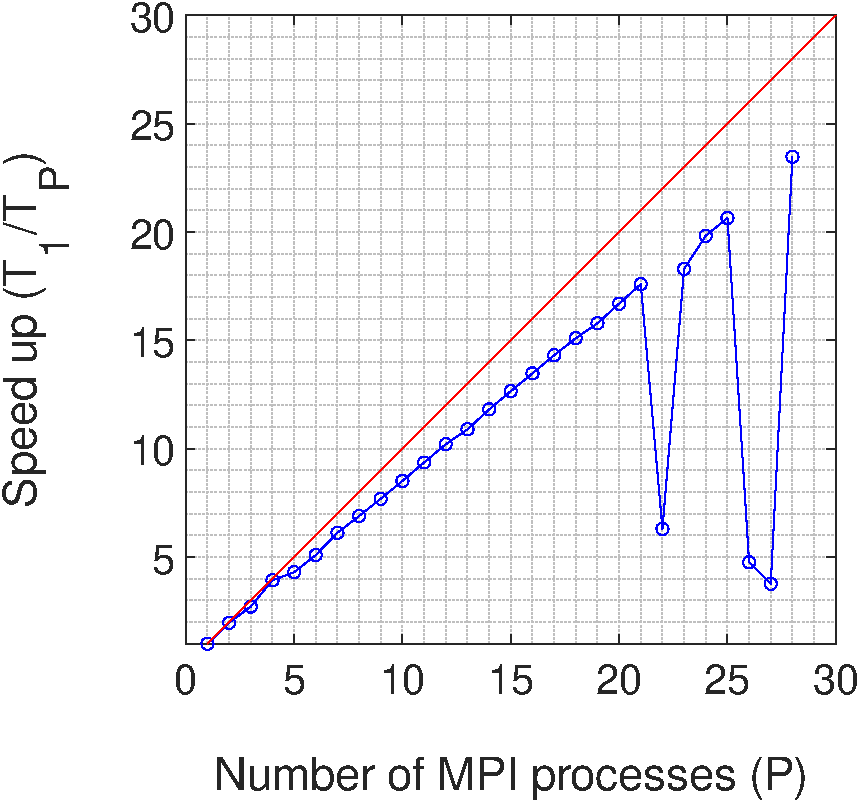
\includegraphics[width=0.5\textwidth]{figures/CMDA3634FA19HW/strongsScalingStudy.pdf}
        \caption{Example of a strong scaling study graph.
        The red line shows the theoretical perfect speedup rate $P=T_1/T_P$.}
        \label{fig_strong_scaling}
    \end{figure}
    \item[Q2.3] (5pts \textcolor{red}{extra credit}) Repeat the above scaling study three more times but on the program with optimized compilation.
    Each of the three compiler flags (\texttt{-O1}, \texttt{-O2}, \texttt{-O3}) should be used in one study.
\end{itemize}
\newpage
\subsection*{Task 3}
Modify your k-means project to run in parallel via MPI.
If you are not satisfied with your own k-means project,
you may use the example k-means project that was provided for HW 9 and the reference code provided for HW10.
\begin{itemize}
    \item[Q3.1] (10pts) Parallelize the cluster centroid calculation using MPI.
    You may use your work from HW 10 or the example solution explained at the top of this assignment.
    \item[Q3.2] (15pts) Parallelize the calculation of the nearest cluster centroid assignment using MPI.
    \item[Q3.3] (15pts \textcolor{red}{extra credit}) Perform optimization and strong scaling studies on your k-means code.
    In other words, repeat Tasks 1 and 2 with your k-means code in place of the cluster-centroid code.
\end{itemize}
While testing your code, you can use any of the data provided for HW 7, 9, or 10.

\subsection*{Submission}

\begin{itemize}
    \item[Q4.1] (5pts) Submit your work as follows.
    \begin{itemize}
        \item Write a report on your results and use \LaTeX{} to typeset it.
        \begin{itemize}
            \item  Your report should include
            \begin{itemize}
                \item \textcolor{red}{All} of the C source files you used, including any that you borrowed from the instructor's example.
                In your report, source files should be nicely formatted with the \texttt{minted} environment.
                \item The table explained in Task 1.
                \item The graphs explained in Task 2.
            \end{itemize}
            \item Upload the PDF and tex files of your report to Canvas.
        \end{itemize}
        \item Submit the C source files of \textcolor{red}{ALL} tasks by pushing them to your Git repository on \href{http://code.vt.edu}{code.vt.edu}
        You may not receive any credit if your code is not in your repository.
        
        Please imitate the directory structure in the instructor's example, shown below.
\begin{verbatim}
HW11/
    makefile
    src/
        mpiCluster.c
        data.c
        [any other source files]
    data/
        mpiClusters.dat
        [any other data files]
    include/
        data.h
        [any other header files]
\end{verbatim}
    \end{itemize}
\end{itemize}
